% Document information
\newcommand{\titleinfo}{Zusammenfassung PMSwEng}
\newcommand{\authorinfo}{Sandro Pedrett}
\newcommand{\version}{1.1}
\newcommand{\versioninfo}{HS21}
% Header
\include{Template/Header}

% Setup Source Code
\lstset{ 
	backgroundcolor=\color{white},   % choose the background color; you must add \usepackage{color} or \usepackage{xcolor}; should come as last argument
	basicstyle=\footnotesize,        % the size of the fonts that are used for the code
	breakatwhitespace=true,         % sets if automatic breaks should only happen at whitespace
	breaklines=true,                 % sets automatic line breaking
	captionpos=b,                    % sets the caption-position to bottom
	commentstyle=\color{ForestGreen},    % comment style
	escapeinside={\%*}{*)},          % if you want to add LaTeX within your code
	extendedchars=true,              % lets you use non-ASCII characters; for 8-bits encodings only, does not work with UTF-8
	frame=single,	                   % adds a frame around the code
	keepspaces=true,                 % keeps spaces in text, useful for keeping indentation of code (possibly needs columns=flexible)
	language=C++,                      % the language of the code
	numbersep=5pt,                   % how far the line-numbers are from the code
	rulecolor=\color{black},         % if not set, the frame-color may be changed on line-breaks within not-black text (e.g. comments (green here))
	showspaces=false,                % show spaces everywhere adding particular underscores; it overrides 'showstringspaces'
	showstringspaces=false,          % underline spaces within strings only
	showtabs=false,                  % show tabs within strings adding particular underscores
	stepnumber=2,                    % the step between two line-numbers. If it's 1, each line will be numbered
	tabsize=2,	                   % sets default tabsize to 2 spaces
	title=\lstname,                   % show the filename of files included with \lstinputlisting; also try caption instead of title
	stringstyle=\ttfamily\color{red!50!brown},
	keywordstyle=\color{blue}\bfseries,
}

% Prüfung open-book für Teil B

% Document
\begin{document}

\section{Vorgehensmodelle}
\subsection{Phasenmodell - Wasserfall-Model}
Es ist einfach, klare Struktur. Jede Phase erzeugt ein Ergebnis, auf dem die nächste Phase aufbaut. Bekannte Vertreter sind Wasserfall oder V-Modell. Jedoch werden Planungsfehler erst spät bemerkt. Risiken werden zu spät erkannt. 
\subsubsection{Wasserfallmodell}
\begin{center}
	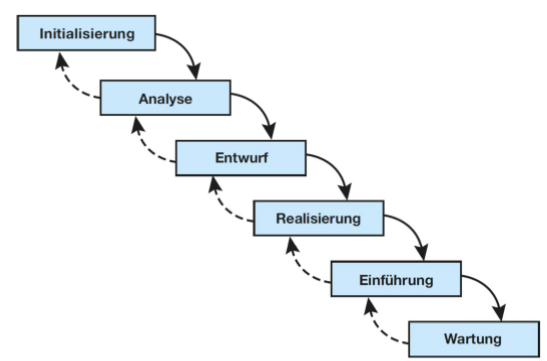
\includegraphics[width=0.6\columnwidth]{Images/Wasserfallmodell}
\end{center}

\subsubsection{V-Modell}
Starke Einbindung der Tests zu jeder Phase. Ähnlich wie bei Wasserfallmodell, auch hier ist eine grosse Erfahrung nötig
\begin{center}
	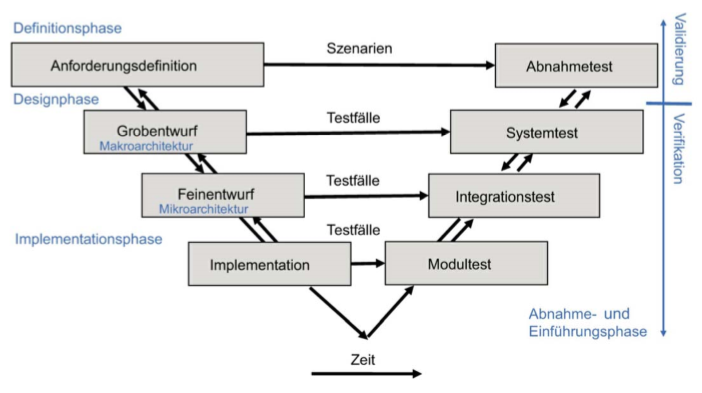
\includegraphics[width=0.6\columnwidth]{Images/v-modell}
\end{center}


\subsection{Agile}
Agile bedeutet "flink, beweglich". Ziel von der Agilen Softwareentwicklung ist es, eine leichtgewichtigen Ansatz mit hoher Flexibilität zu gewährleisten zB um Änderungen gut und schnell aufnehmen zu können ohne weitere Probleme. Agile Projekte werden vorallem für Software-Projekte eingesetzt, da Software-Entwicklung sehr flexibel ist. Für grosse und langlebige Projekte mit zB Regolatorischen-Anforderungen nicht geeignet (tailoring Notwendig aka. \textbf{Hybrid-Modell}).

\subsubsection{Spiralenmodell}
Ein iterativer/inkrementeller Vorgehen. Erlaubt kontinuerliche Lernkurven und eine schnelles Feedback vom Kunden. Ergebnisse der Zyklen wie Anforderung oder Architektur werden bei jeder Iteration verfeinert und Risiken frühzeitig erkannt.
\begin{center}
	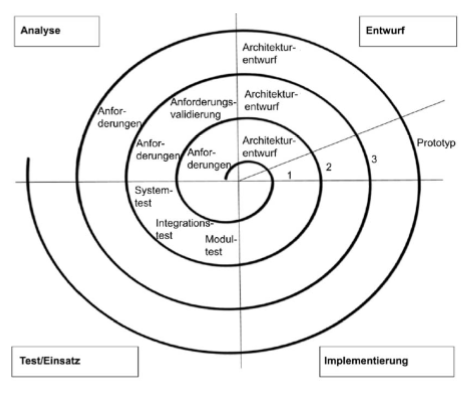
\includegraphics[width=0.6\columnwidth]{Images/spiralmodell}
\end{center}

\subsubsection{Scrum}
Ein agiles und sehr bekanntes Vorgehensmodel ist Scrum. Es werden dabei grob in drei Phasen unterteilt:
\begin{enumerate}[nosep]
	\item Grobplanung: Allgemeine Ziele festlegen und Software-Architektur planen
	\item Inkrementelles Entwicklung der Software
	\item Projektabschluss, Dokumentation werden vervollständigt und Lehren aus dem Projekt werden gezogen.
\end{enumerate}

In Scrum sind folgende Keywords unabdingbar:\\
\begin{tabular}{lm{6cm}}
	\textbf{Backlog} & Eine art To-Do Liste (Ansammlung von UserStories) die das Scrum-Team abarbeitet muss. \\
	\textbf{User Story} & Beschreiben Aufgaben, welche vom System gefordert werden. Sie müssen nicht von Anfang an detailiert sein, müssen aber bei der Umsetzung genau spezifiziert sein. \\
	\textbf{Product Owner} & Ein Kunde oder auch Projektmanager. Definiert was das Produkt können muss \\
	\textbf{Sprint} & Eine Entwicklungsiteration, Dauer in der Regel zwischen 2-4 Wochen. Definiert welche UserStories in der Itaration umgesetzt werden (Diese UserStories dürfen nicht mehr geändert werden) \\
	\textbf{Scrum} & Tägliches Meeting des Scrum-Teams, bei dem Fortschritt, Probleme und priorität überprüft werden.\\
	\textbf{Scrum Master} & Stellt sicher, dass Scrum-Prozess eingehalten wird. Er ist nicht der Projektleiter! \\
	\textbf{Velocity} & Eine Schätzung, wie viel vom Backlog ein Team in einem Sprint abdecken kann. Bietet eine Messung für die Leistungsbewertung des Teams.
\end{tabular}

\subsection{Hybrid-Modell}
Keine Modell ist perfekt, in der Praxis werden daher die Vorgehensmodelle vermischt und je nach Firma unterschiedliche angewandt. Im folgenden ein Beispiel
\begin{center}
	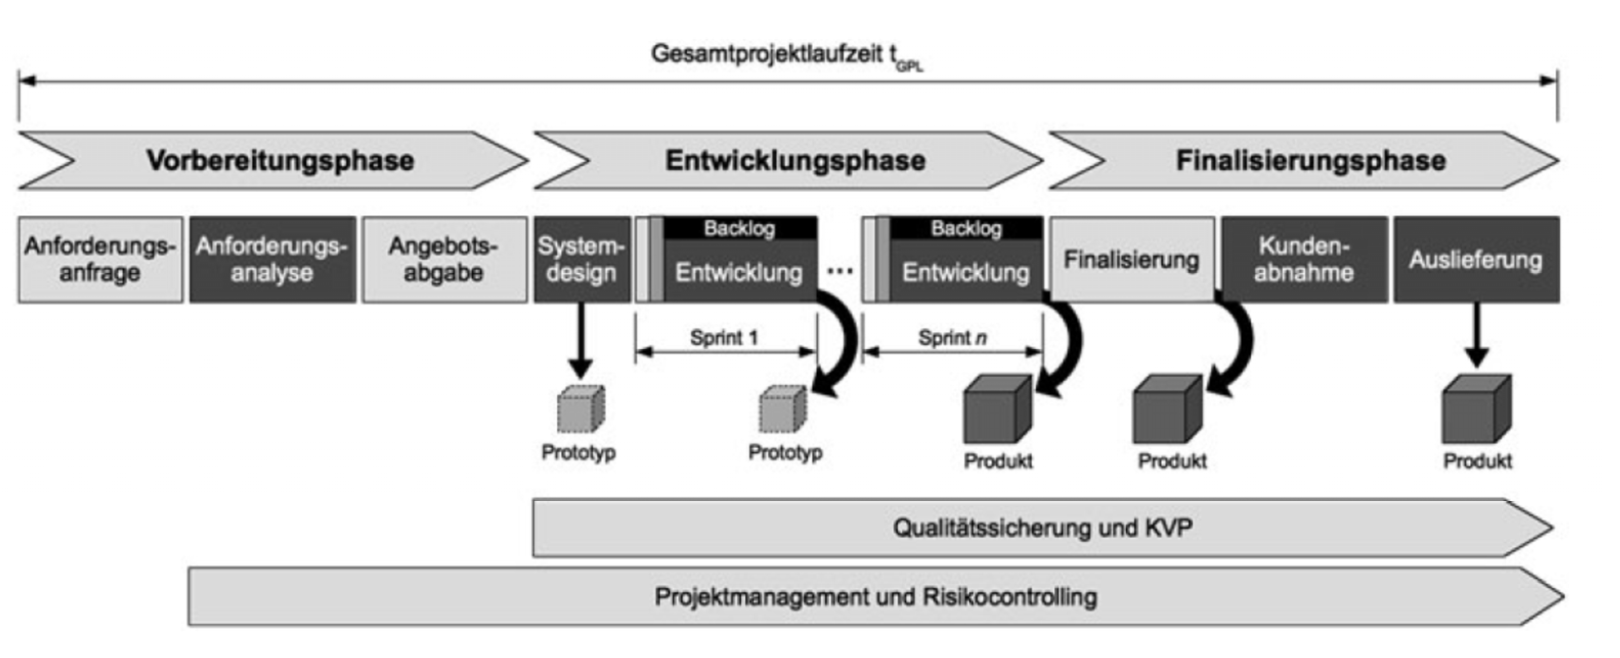
\includegraphics[width=\columnwidth]{Images/vorgehensmodell_beispiel}
\end{center}
\newpage
\section{Requirements-Engeneering}
Das \textbf{Lastenheft} beschreibt die gesamte Funktionalität, die eine Software erfüllen soll, und dient als Grundlage für die Einholung von Angeboten und wird aus sicht des Auftraggebers geschrieben. Das \textbf{Pflichtenheft} stellt die Softwarelösung des Anbieters dar und beschreibt, wie die im Lastenheft gewünschten Funktionen umgesetzt werden.

\subsection{Stackholder}
Stackholder sind Persona, welche mit dem System interagieren. Dies können einzelene Personen oder auch Gruppen bzw. andere Sofware-Teile sein. Sie müssen sehr sorgfälltig evaluiert werden, um nachfolgend die Anforderungen sauber zu definieren.

\subsection{Kontextabgrenzung}
Stellt sicher, das ein System von der Umwelt abgeschottet ist. Oft wird zur Übersicht ein Diagram erstellt, welche die Grenzen klar darstellt. Folgendes Beispiel für einen SPICE Simulator, welcher drei Sub-Systeme beinhaltet. Jedes dieser Sub-System kommuniziert über einen definierten Kanal.
\begin{center}
	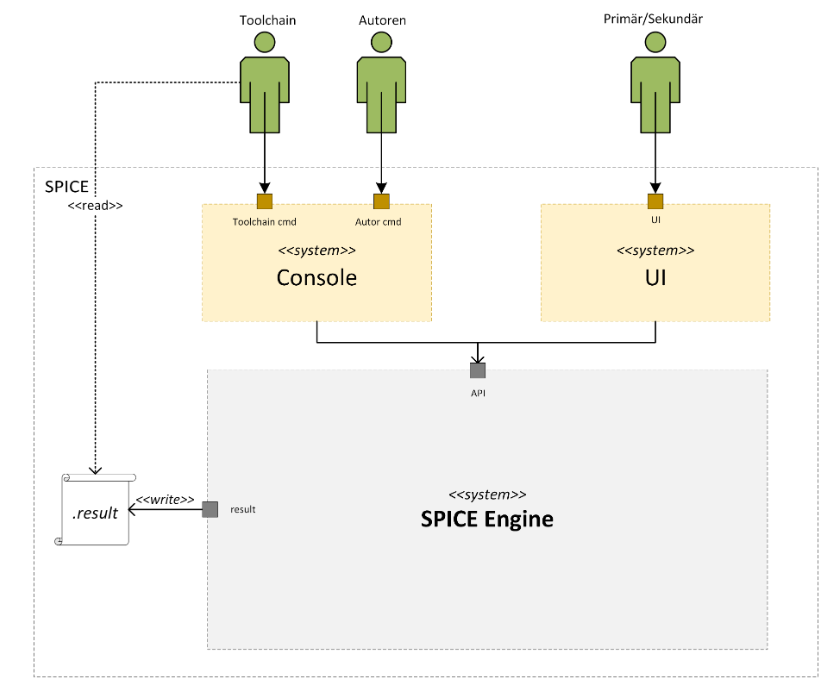
\includegraphics[width=\columnwidth]{Images/kontextabgrezung}
\end{center}

\subsection{Anforderungen}
Anforderungen werden häufig in folgende Gruppen unterteilt: 
\begin{itemize}[nosep]
	\item Funktionale Anforderungen
	\item Nichtfunktionale Anforderungen
	\item Rahmenbedingungen
\end{itemize}

\subsubsection{Nichtfunktionale Anforderungen} sind jene, welche gefodert werden, aber keine neuen Funktionen beiten. zB Qualitätsanforderungen (Genauigkeit, Verfügbarkeit, Zuverlässigkeit). Diese Anforderungen betreffen meist mehrere Funktionalen Anforderungen und können sich auch gegenseitig beeinflussen (Sicherheit vs Benutzerfreundlichkeit)

\subsubsection{Funktionale Anforderungen} lassen sich gut mittels Use-Case Diagram beschreiebn. Sie definieren welche Eigeschaften ein System hat und welche Funktionalität erwartet werden kann. zB Tempo Messen
\begin{center}
	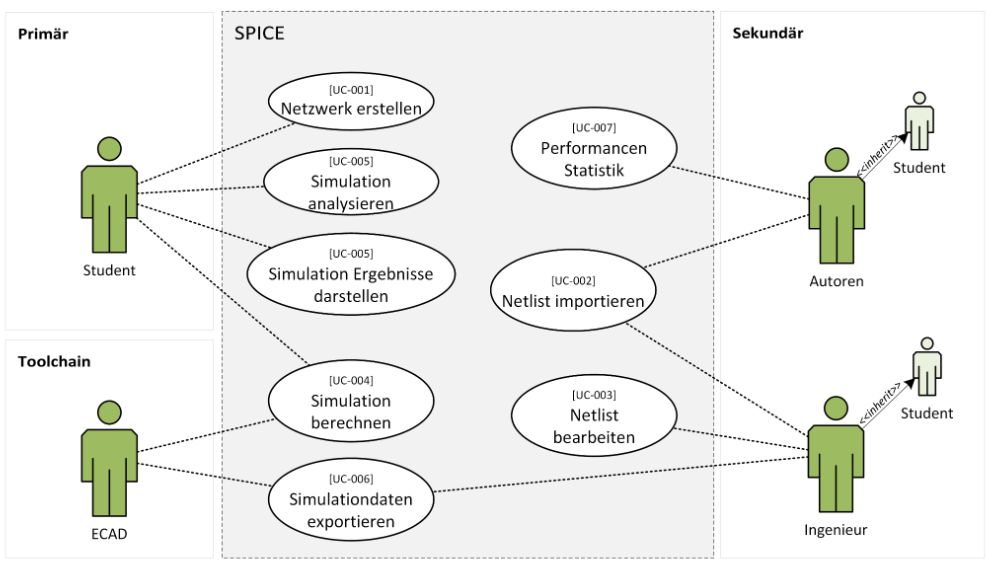
\includegraphics[width=\columnwidth]{Images/usecase}
\end{center}


\subsubsection{Rahmenbedingungen} sind im gegensatz zu Anforderungen Einschränkungen. \underline{Technische} Rahmenbedingungen sind zB \textit{Software muss auch Windows lauffähig sein}, \textit{Git muss eingesetzt werden}. etc. Des weiteren sind \underline{organisatorische} Rahmenbedingungen zB \textit{Team ist 4 Mann gross}. Rahmenbedingungen können grundsätzlich nicht geändert werden und vordern oft vordefinierte Lösungen (Was gute Anforderungen auf keinen Fall tun sollten).

\subsubsection{Vorgehen}
Das vorgehen, um gute Anforderungen zu definieren ist schwierig. Oft werden Stakeholder mittels Interview befragt oder Selbstaufschreibung.  
\begin{center}
	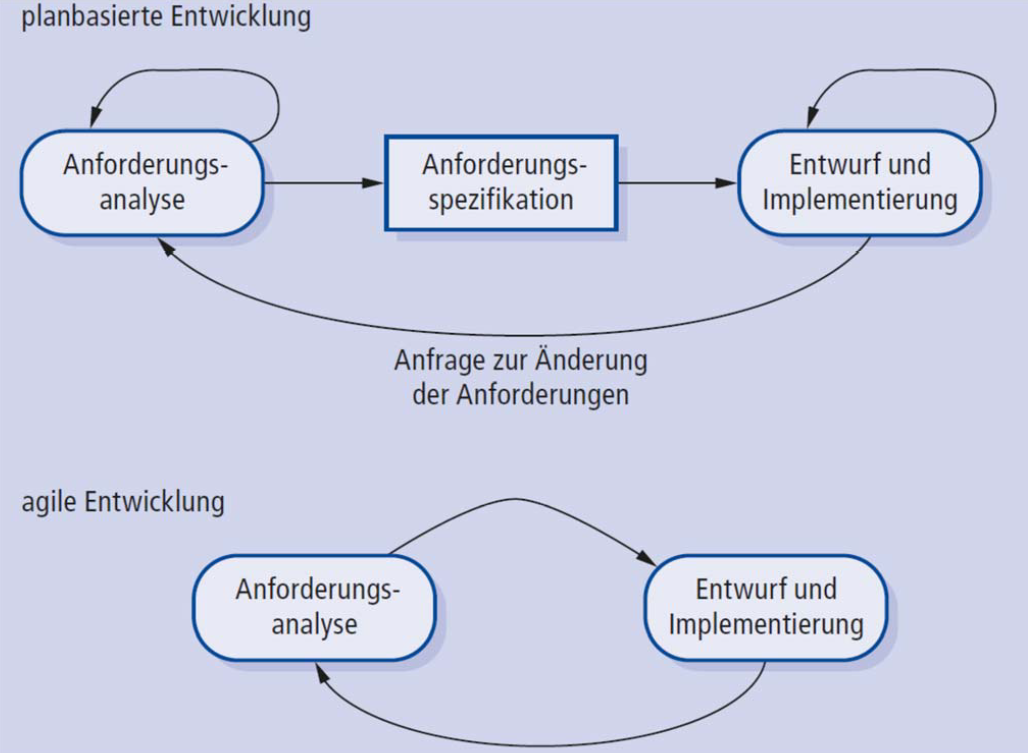
\includegraphics[width=\columnwidth]{Images/requirements_engeneering}
\end{center}

~\\ ~\\
\textbf{Tips} für Anforderung: Anforderungen müssen überprüfbar, eindeutig, vollständig, realisierbar und gültig sein.
\begin{center}
	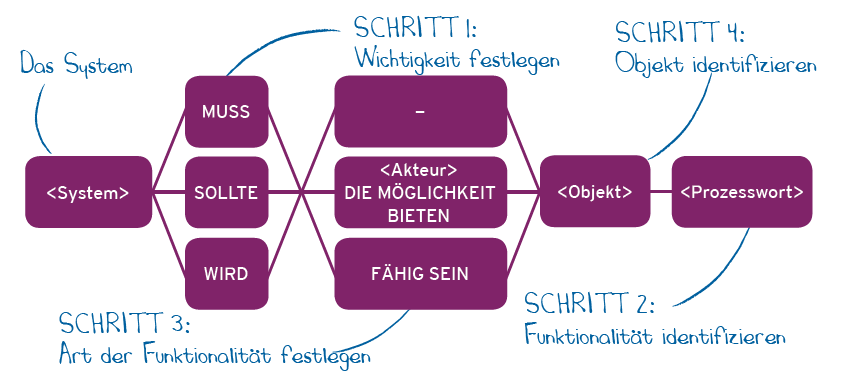
\includegraphics[width=\columnwidth]{Images/schablone}
\end{center}


\section{Projektplanung}
\subsection{Plangesteuert}
In der klassischen Projektplanung werden folgende Schritte durchgeführt:\\
\begin{tabular}{lm{5.5cm}}
	\textbf{Strukturplan} & Der Strukturplan legt fest, wie ein Projekt organisiert bzw. welches Vorgehen gewählt wird. Das Projekt wird mithilfe der definierten Anforderungen in \textbf{Arbeitspakete} unterteilt (In Scrum könnten das zB User Stories sein). \\
	\textbf{Aufwandschätzung} & Einzelene Arbeitspakete (UserStories) werden abgeschätzt.\\
	\textbf{Arbeitsplan} & Die voneinander abhängigen Arbeitspakete werden vernetzt und oft auch an Entwickler zugewiesen. (zB mit Gantt-Diagramm) \\
	\textbf{Kostenplanung} & Kosten werden abgeschätzt \\
	\textbf{Risikomanagement} & Risiken bewertet und allfällig behoben
\end{tabular}

\subsection{Agil}
In der moderneren Projektplanung, bei der nach einem Agilen Prinzip gearbeitet wird, sind folgende Schritte durchzuführen:
\begin{tabular}{lm{5.5cm}}
	\textbf{Releaseplanung} & Welche Epics (Gruppierung von UserStories) werden für welche Version geplant. \\
	\textbf{Iterationsplanung} & Welche UserStories müssen in der nächste Iteration umgesetzt werden \\
	\textbf{Aufwandschätzung} & UserStories müssen abgeschätzt werden \\
	\textbf{Aufgabenplanung} & UserStories in Tasks unterteilen. zB für UserStore: \textit{Tempo Messen} mehrere Task umgesetzt werden (Sensor auslesen, Filtern, Darstellen usw)
\end{tabular}

\subsection{Aufwandschätzung}
Um Aufwände zu schätzen muss Anforderung bzw Pflichtenheft so detailiert wie möglich sein. Arten zur Schätzung:
\begin{itemize}[nosep]
	\item Bauchgefühl
	\item Algorithmisch - Eine Formel suchen und pro Task anwenden
	\item Vergelichen - Anhand abgeschlossener Projekte vergleiche ziehen
	\item Exportenbefragung - Know-How von Mitarbeitern nutzen
\end{itemize}

In der klassischen Projektplanung werden Stunden pro Task geschätzt. Für agile Methoden können auch StoryPoints pro UserStory vergeben werden. Ziel ist es, eine Stundenunabhängige Einheit zu schaffen (Dies löst das Problem, dass ein Task von Mitarbeiter A nicht gleichschnell gelöst wird wie von Mitarbeiter B). Jeder Mitarbeiter weiss, wieviele StoryPoints er pro Itartion erledigen kann.
\section{Git}
Ein VCS (Version-Control System) ist ein System, das zur Erfassung von Änderungen an Dokumenten oder Dateien verwendet wird. Alle Versionen werden in einem Archiv mit Zeitstempel und Benutzerkennung gesichert und können später wiederhergestellt werden. Ein verbreitetes VCS ist in der Software Enwicklung \textbf{Git}.

\subsection{Git Übersicht - Vereinfacht}
In einem Git-Repository (aka. Git Projekt) hat jede Datei eines der drei Zustände.\\
\begin{center}
	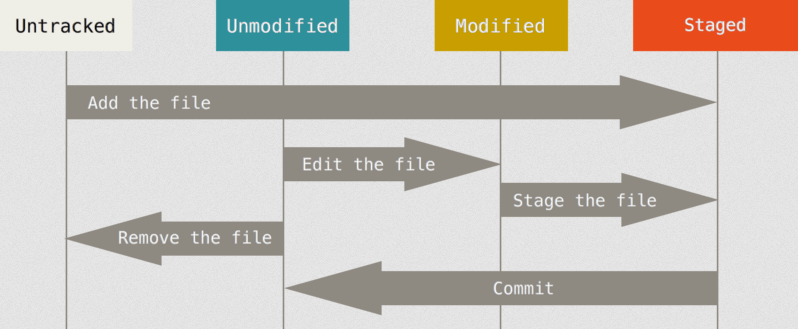
\includegraphics[width=\columnwidth]{Images/git.png}
\end{center}
\begin{tabular}{p{9cm}}
	\textbf{Untracked}, Datei wird von git irgnoriert \\
	\textbf{Unmodified}, Datei ist nicht bearbeitt worden (in git gesichert)\\
	\textbf{Modified}, Datei ist bearbeitet wird aber nicht gesichert\\
	\textbf{Staged}, Datei ist bearbeitet und wird beim nächsten Commit gesichert
\end{tabular}
~\\~\\
Um Änderungen von Dateien in git zu Speichern, müssen diese als staged eingetragen sein. Beim Speichern wird ein \textbf{Commit} erstellt und dem letzten Commit hinzugefügt. Dadurch entsteht eine Liste von Änderungen aka. History. Zu jedem Commit kann gesprungen werden, und neue Commits hinzugefügt werden. Dadruch entsteht \textbf{Branches}, welcher unabhängig von anderen verändert werden können. Der \textbf{HEAD} zeigt immer auf den aktiven Commit.
\begin{center}
	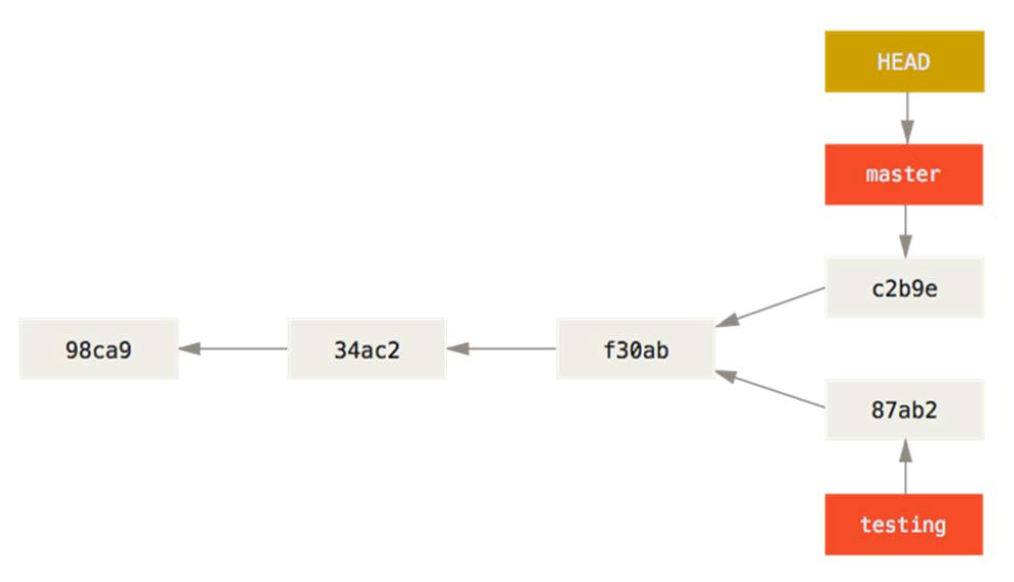
\includegraphics[width=\columnwidth]{Images/branches}
\end{center}


Commits können an eine anders Git-Repository auf zB einem Server (im folgenden als \textbf{Remote} bezeichnet) geschickt bzw heruntergeladen werden.
\begin{center}
	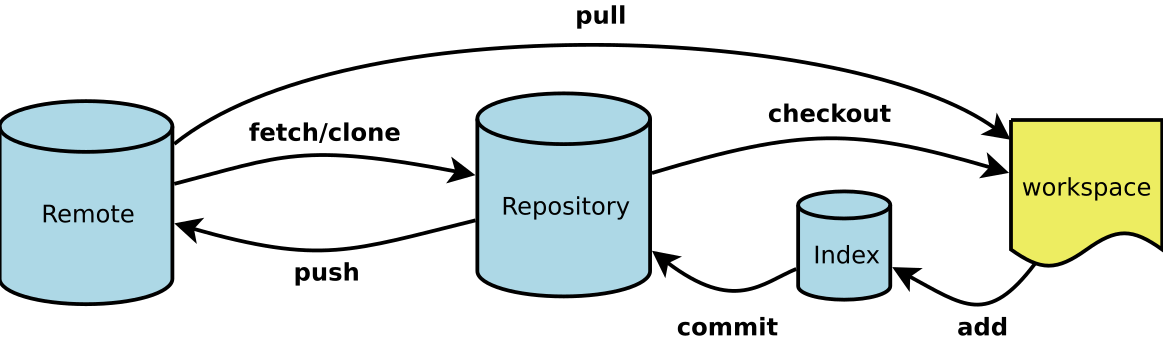
\includegraphics[width=\columnwidth]{Images/remote}
\end{center}


\section{Testen}
Getestet wird auf verschiedenen Ebenen. Je nach Ebene, machen unterschieliche Tests sinn. Je mehr Testen, desto besser. Jedoch sollen Prüfkosten pro entdecktem Fehler eine festgelegte Grenz nicht überschreiten oder mit den Testspezifikationen keine Fehler mehr gefunden werden.
\begin{center}
	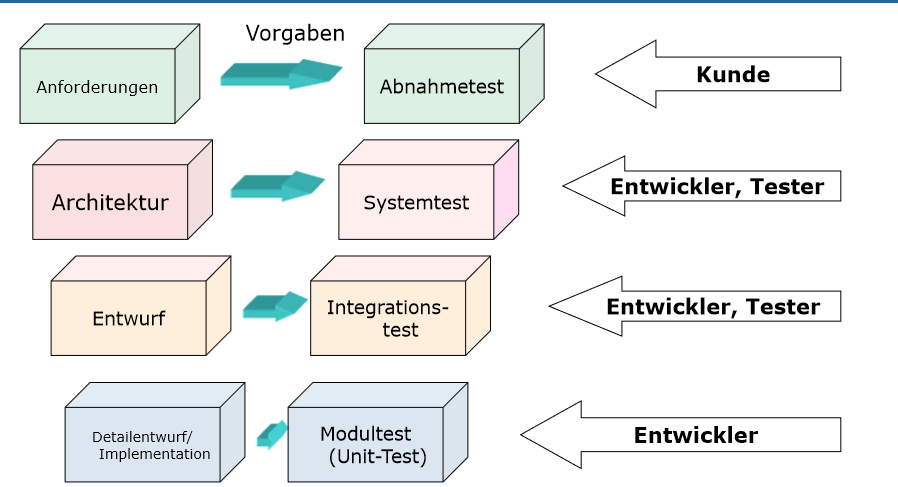
\includegraphics[width=\columnwidth]{Images/testen}
\end{center}

Dabei wird unterschieden zwischen \textbf{Verifikation}: Überprüfen ob die Vorgaben erfüllt sind (Sind alle Anforderungen im Pflichtenheft umgesetzt) und \textbf{Validierung}: Überprüfen ob Anforderungen auch ihren Nutzen erfüllen.

\subsection{Statisch vs Dynamisch Test}
Bei dynamischen Tests wird SUT (Software under Test) ausgeführt zB mittels UnitTests. Bei statische Tests muss SUT nicht aufgeführt werden zB Code-Analyse oder auch Reviews.

\subsubsection{Review}
Bei einem Review wird SUT von einem festgelegten Team auf Fehler untersucht. Fehler werden in einem Review-Bericht gesammelt und am schluss unterzeichnet. Typisches vorgehen bei einem Review:
\begin{center}
	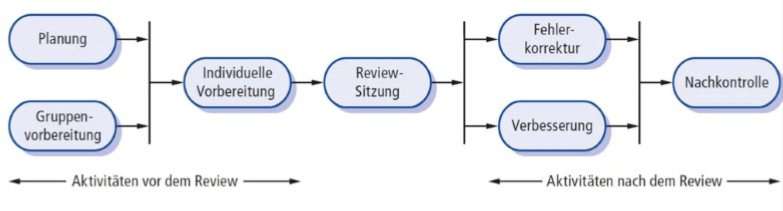
\includegraphics[width=\columnwidth]{Images/review}
\end{center}


\subsection{Black-Box Test}
Beim \textbf{Black-Box} Test gibt es keine Kenntnisse über das Innenleben. Nur Inputs und Outputs können getestet werden. 

\subsubsection{Äquivalenzklassen}
Bei diesem Verfahren werden Wertebereiche definiert, bei dem SUT das gleiche Verhalten erwartet wird. Anschliessend wird pro Klasse ein Testfall erstellt.~\\
\textbf{Beispiel} 

\begin{center}
	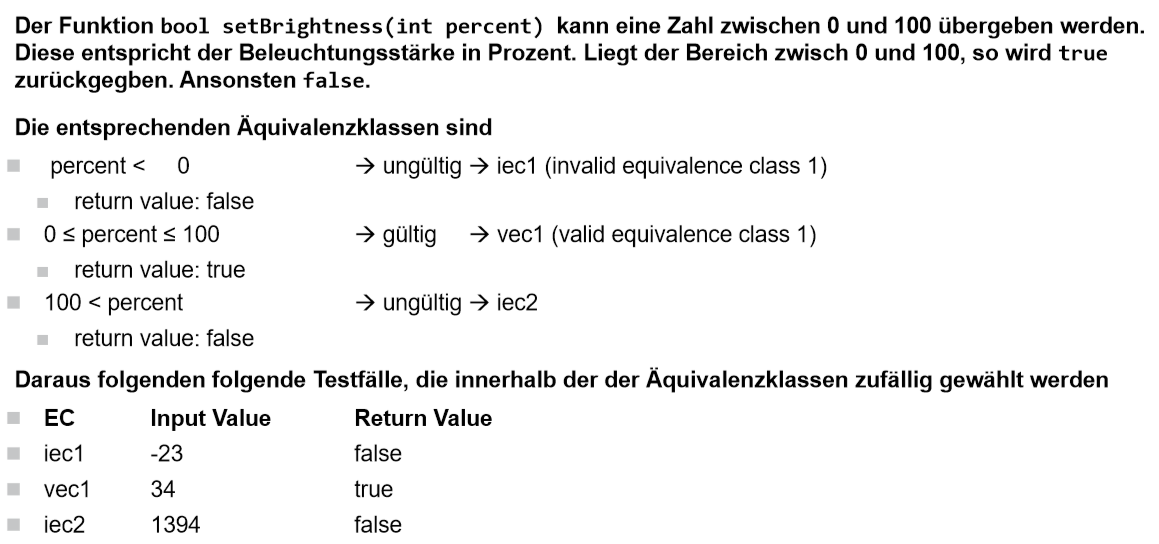
\includegraphics[width=\columnwidth]{Images/aequivalenzklassen}
\end{center}

\subsubsection{Grenzwertanalyse}
Diese Methode kann Äquivalenzklassenmethode erweitern. Die Erfahrung zeigt, dass Fehler häufig bei den Grenzen zwischen Äquivalenzklassen entstehen.
\begin{center}
	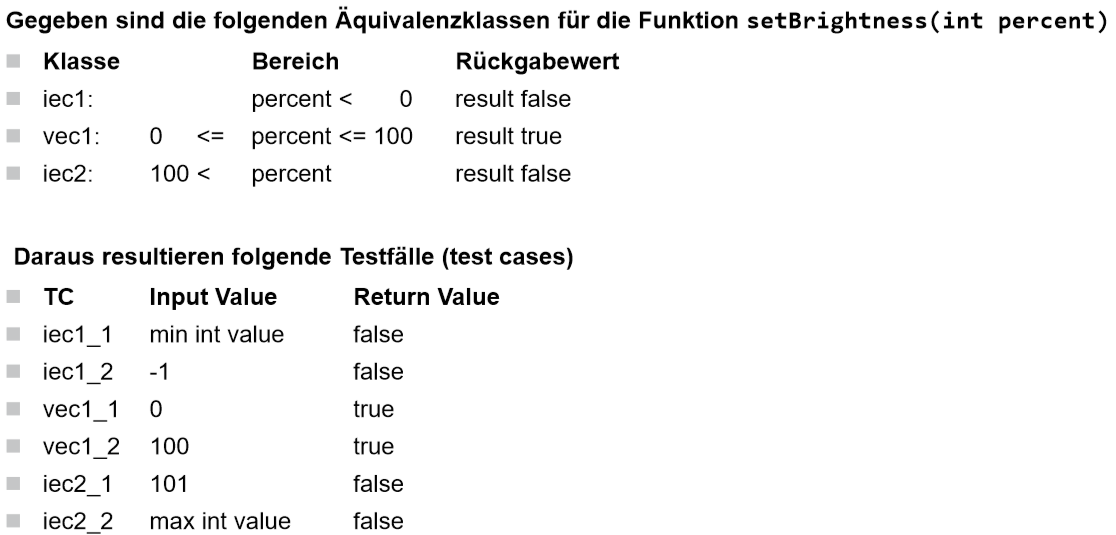
\includegraphics[width=\columnwidth]{Images/grenzwert}
\end{center}

\subsection{White-Box Test}
 Im gegensatz zur Black-Box ist das Innenleben bei \textbf{White-Test} bekannt. Dadurch ist es theoretisch möglich, alle Möglichkeiten zu testen. Dies wird in einem Code-Coverage bericht festgehalten.
 
\subsection{Testframework - googletest}
Mittels Testframework können Software Tests automatisiert werden. 
\begin{lstlisting}
TEST(KlasseName, TestMethodName) {
	MyClasse c1;
	ASSERT_EQ(c1.getValue(), 1);
}
\end{lstlisting}
Weitere Asserts:
\begin{itemize}[nosep]
	\item ASSERT\_EQ,NE,GT,GE,LT,LE(val1, val2)
	\item ASSERT\_TRUE,FALSE(condition)
	\item ASSERT\_STREQ,STRNE(str1, str2)
	\item EXPECT\_FLOAT\_EQ(val1, val2)
\end{itemize}
\section{Doxygen}
Zweck von Software Code Dokumentation ist die Wissensicherung, Kommunikation und das sichtbarmachen des Projektfortschrittes. Mittels Doxygen kann Code dokumentiert und ein entsprechends Dokument erzeugt werden. Damit findet man nicht Dokumentierte Parameter leichter und die Dokumentation bleibt konsistent mit Software. (WICHTIG: Doxygen ersetzt nicht Software-Dokumentation ansich!). 
\begin{center}
	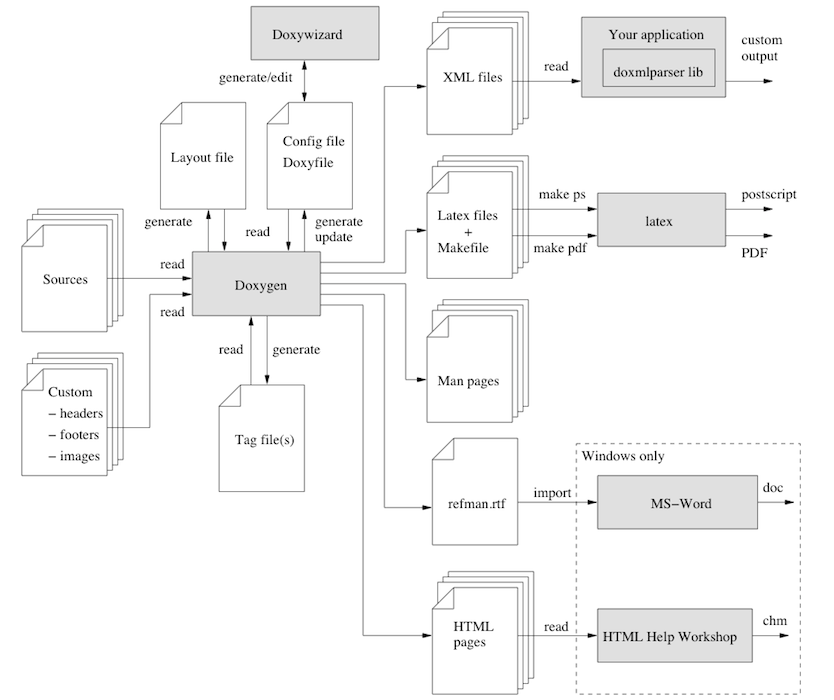
\includegraphics[width=\columnwidth]{Images/doxygen}
\end{center}

Die Wichtigsten Doxygen Funktionen (doxygen kann mittels \textit{doxygen.exe -g} eine neue Konfigurations Datei erstellen und mit  \textit{doxygen.exe ConfigFileName} gestartet werden):
\begin{itemize}[nosep]
	\item brief
	\item param
	\item pre*
	\item post*
	\item return
\end{itemize}
\begin{lstlisting}
///
/// \brief Calculates the optimal values for R1 and R2. The base formula
/// behind this calculation is \f$u1=u2 {r2 \over r2+r1}\f$.
/// \pre \p u1 > \p u2
/// \pre \p lowerRTh < \p upperRTh
/// \param u1 Value for U1 in V
/// \param u2 Value for U2 in V
/// \param lowerRTh set the lower bound for resistor value output
/// \param upperRTh set the higher bound for resistor value output
/// \param resDecade gives the resister e-decade on which the resistor are
/// calculated
///
virtual void calc(double u1, double u2, double lowerRTh, double upperRTh,
const EDecade& resDecade);
\end{lstlisting}
\section{Event Handling}
Reaktive Systeme sind per definition asynchron, dH sie treten zu einem beliebigen Zeitpunkt ein.

\subsection{C-Implementation}
\textbf{main.h}
\begin{lstlisting}
#include "framework.h"
	
void onCallback(int param) {
	printf("Callback executed");
}
	
int main(void) {
	registerCallback(onCallback);
	run();
}
\end{lstlisting}

\textbf{framework.h}
\begin{lstlisting}
typdef void (*Callback)(int);

static Callback notify;

void registerCallback(Callback c) {
	notify = c;
}

void run() {
	if (notify != 0) {
		notify(4);
	}
}
\end{lstlisting}

\subsection{C++ Implementation I}
\textbf{main.h}
\begin{lstlisting}
#include "framework.h"

class Part {
public: 
	void onCallback(int param) {
		printf("Callback executed");
	}
};

int main(void) {
	Part p;
	Framework f;
	
	f.registerCallback(p, &Part::onCallback);
	f.run();
}
\end{lstlisting}

\textbf{framework.h}
\begin{lstlisting}

class Part; // Class Forward-Declaration

class Framework {
public:
	void registerCallback(Part& p, void (Part::*pFct)(int)) {
		part = &p;
		callback = pFct;
	}
	
	void run() {
		(part->*callback)(5);
	}

private:
	Part* part;
	void (Part::*callback)(int);
};
\end{lstlisting}

\subsection{C++ Implementation II}
\textbf{main.h}
\begin{lstlisting}
#include "framework.h"

class Part : public IPart {
public: 
	virtual void onCallback(int param) override {
		printf("Callback executed");
	}
};

int main(void) {
	Part p;
	Framework f;
	
	f.registerCallback(p);
	f.run();
}
\end{lstlisting}

\textbf{framework.h}
\begin{lstlisting}

class IPart {
public:
	virtual void onCallback(int param) = 0;
	virtual ~IPart() {};	
};

class Framework {
	public:
	void registerCallback(Part& p) {
		part = &p;
	}
	
	void run() {
		if (part != nullptr) {
			part->onCallback(5);
		}
	}
	
	private:
	IPart* part;
};
\end{lstlisting}
\section{Library/Framework}
\textbf{Library} stellt bereits fertig implementierte Funktionalitäten zur Verfügung und der Benutzer kann diese normalerweise nicht überschreiben. Diese können über API aufrufe (aka Methoden aufrufe) genutzt werden zB \textit{std::abs(...)}, wobei std die Standard-Library von c++ ist. \textbf{Framework} bietet hingegen ein Gerüst an, welches vom Benutzer erweitert werden kann zB QT oder .NET. In der Umgangssprache sind diese zwei Begriffe äquivalent.
\begin{center}
	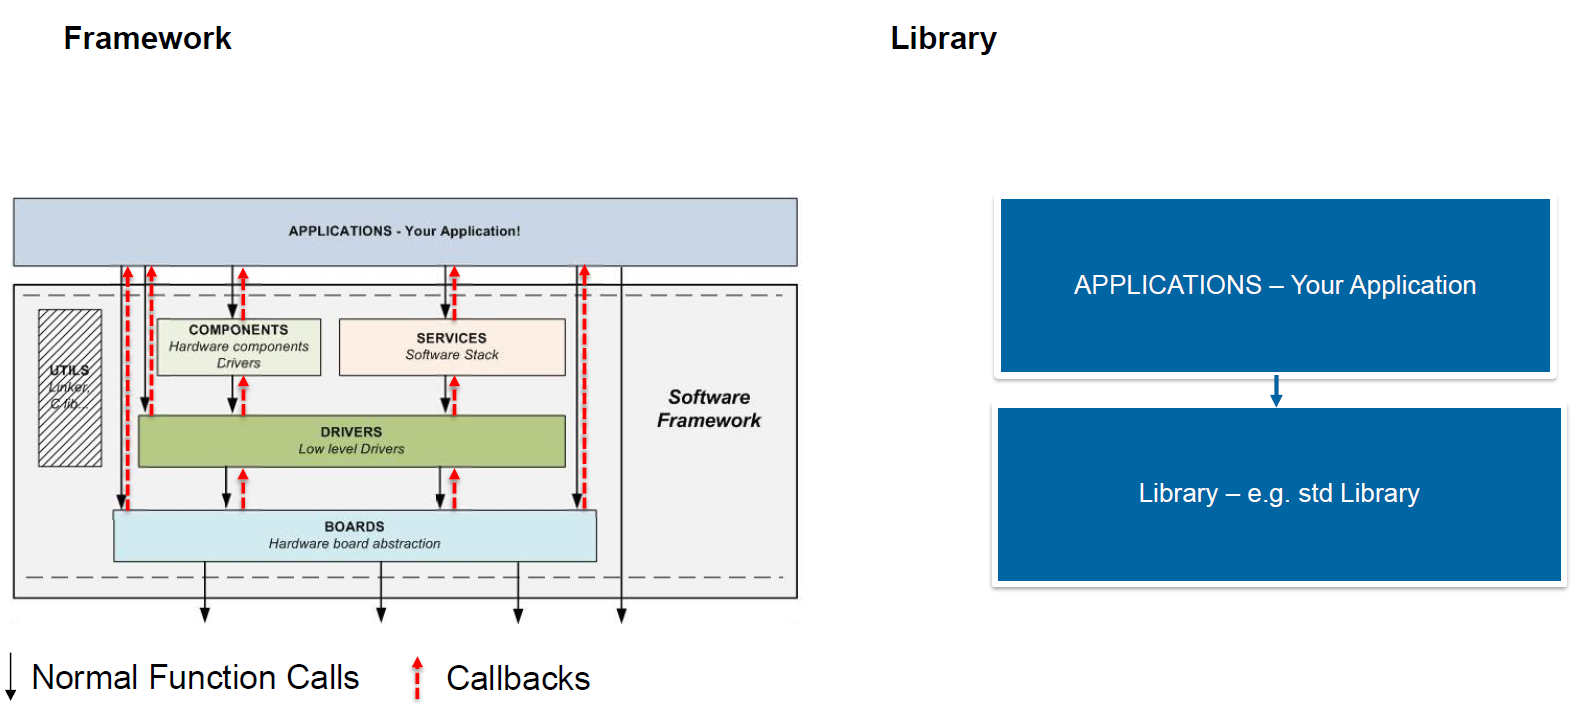
\includegraphics[width=\columnwidth]{Images/framework_library}
\end{center}


\subsection{Static vs Shared}
In c++ werden Klassen beim Kompilieren in Object Files umgewandelt. Eine Sammlung von Object-Files ergeben eine Library (Bibliothek) welche beim Linken Statisch oder als Shared hinzugefügt werden. Der Output hängt vom gewählten Target ab (im folgenden zB Windows). 

Jede \textbf{Shared-Library} endet auf Windows mit *.dll (Dynamic Link Library) und werden nach dem Programmstart geladen. Dies macht die *.exe sehr viel kleiner, wenn zB DLL zwischen Applikationen geteilt werden. Bei nicht vorhandenen DLL kann die Applikation jedoch nicht gestartet werden. Bei \textbf{Static-Library} werden die Object-Files direkt in die *.exe gelinkt, was diese grösser macht, jedoch müssen beim Programmstart nicht zusätzliche Libs geladen werden (bzw können nicht vergessen werden).

\newpage
\begin{landscape}
	\begin{center}
		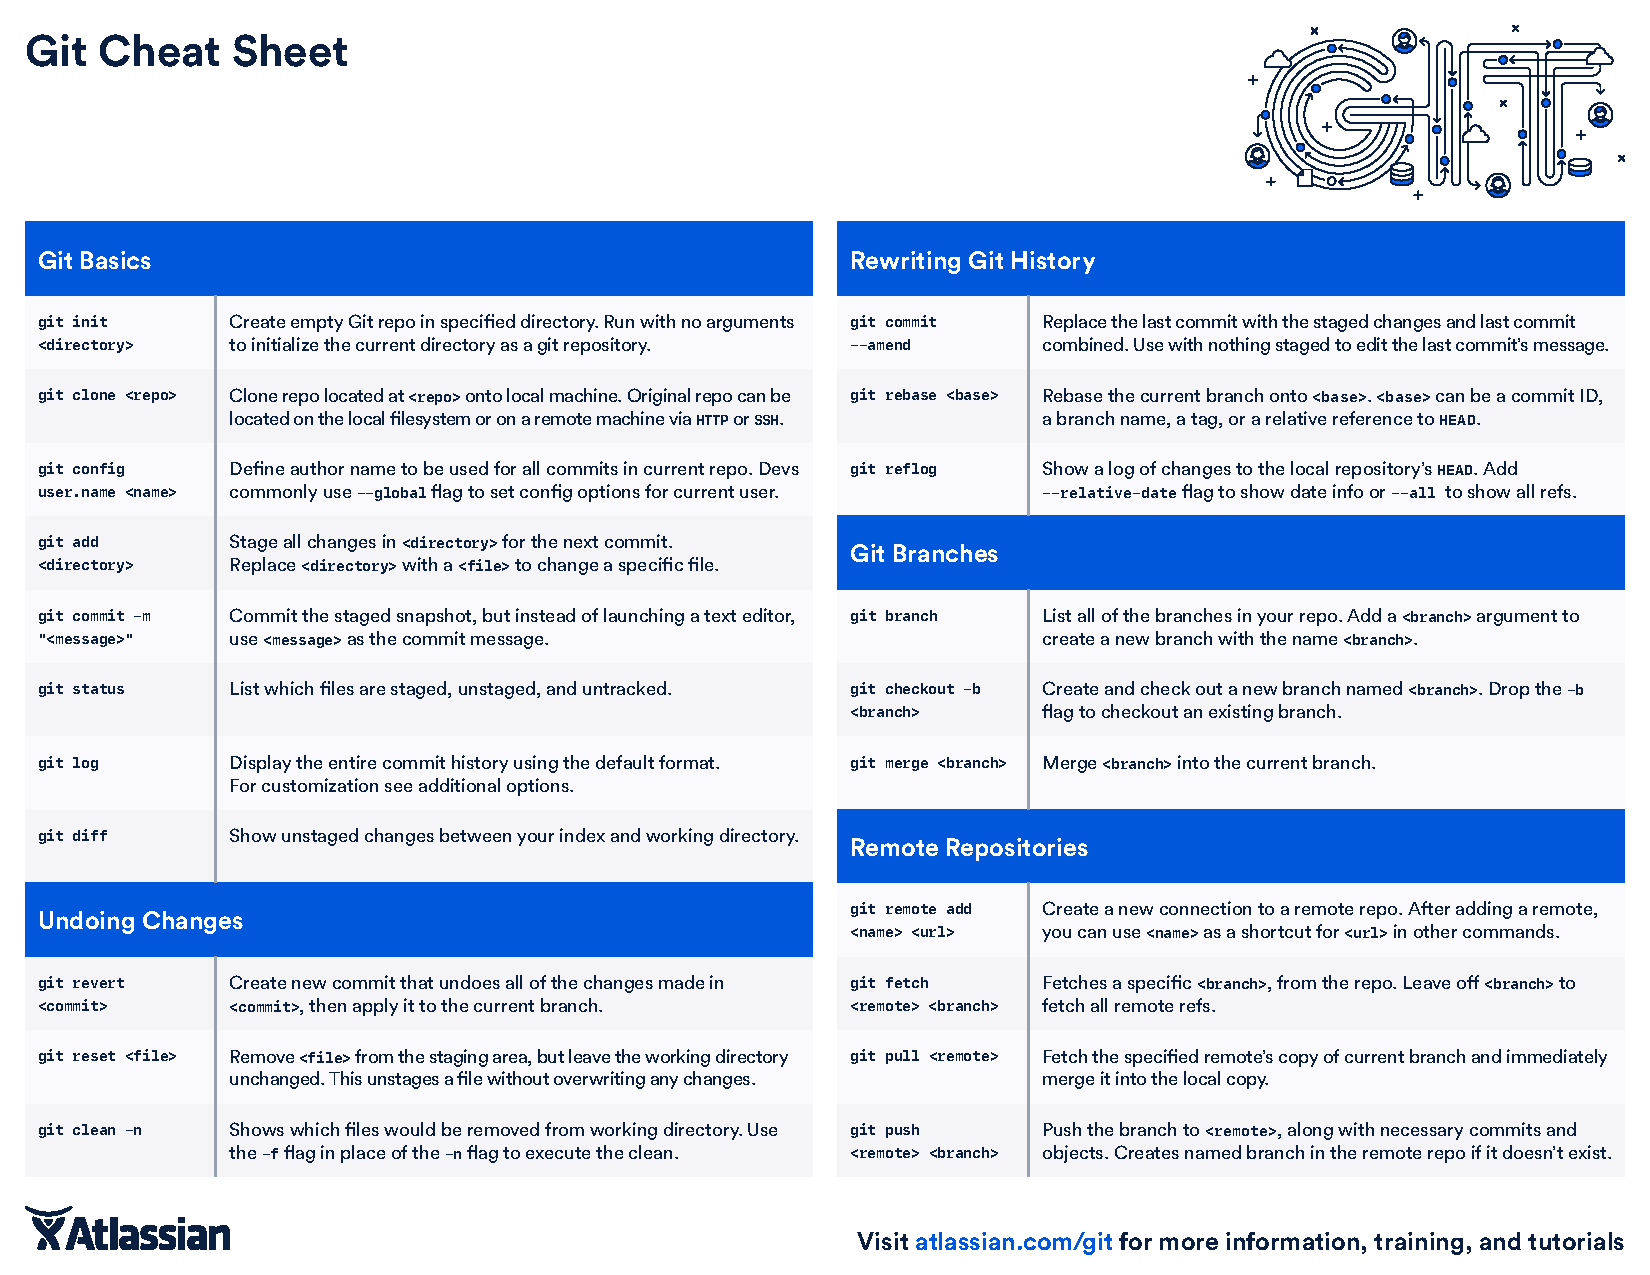
\includepdf[pages=-2, scale=0.9, landscape=true]{Images/git.pdf}
	\end{center}
\end{landscape}


\end{document}